\chapter{Requisitos}
Neste trabalho, procuramos identificar um \textit{backend} conveniente para o desenvolvimento de aplicações \textit{mHealth}. Para isso, vamos definir um sistema-alvo, que requer uma arquitetura tipica de uma solução de \textit{mHealth}. O objetivo é partir de um cenário concreto para extrair requisitos que possam validar a arquitetura escolhida.
\section{Visão geral do sistema a desenvolver}
% nesta secção, apresentar o PRODUTO proposto: um sistema para apoiar projetos de I&D que incluem recolha de dados fisiológicos, que podem ocorrer em laboratório, como em ambulatório Identificar os atores envolvidos e as suas motivações 
O produto proposto é um sistema que permite a recolha de dados fisiológicos de pessoas e a respetiva revisão dos dados recolhidos por parte dos profissionais, responsáveis pelo estudo. A recolha pode ocorrer em laboratório ou em ambulatório, isto é, os participantes podem recolher estes dados presencialmente ou remotamente. Um dos objetivos deste sistema é apoiar projetos de \gls{ID} que incluem componentes de análise da fisiologia humana.
\par 
O sistema será composto por uma aplicação móvel que tem como objetivo principal recolher dados dos sensores, e uma aplicação \textit{web} para visualizar esses dados recolhidos. O sistema irá contemplar então dois atores distintos:
\begin{itemize}
  \item Revisor/Investigador que tem como objetivo rever dados inseridos pelos diferentes participantes num estudo.
  \item Participante(alvo de estudo) que tem como função recolher dados vitais e acelerómetro para posteriormente serem revistos pelo revisor/investigador.
\end{itemize}

O dispositivo com sensores utilizado poderá ser o \textit{VitalJacket} \cite{vj} e os dados fisiológicos recolhidos poderão ser a frequência cardíaca, \gls{ECG} e acelerómetro. Poderá ser utilizado este dispositivo pois como já fez parte de outros estudos, é um equipamento válido e permite recolher os tipos de dados que pretendemos. \par 
A acelerómetro está integrado no \textit{VitalJacket} e a sua integração deve-se à facilidade com que este sensor aparece hoje dia em \textit{smartphones}, \textit{smartwatchs} e \textit{bracelets}. É uma variável adicional, típica das aplicações móveis, mas ausente dos sistemas de dados clínicos clássicos.  
\newpage
\section{Casos de Utilização na Colheita de Dados}

Na figura \ref{f:usecaseandroidapp} podemos visualizar um diagrama com os casos de utilização (cenários-objetivo) da aplicação móvel. O principal ator desta aplicação é o participante que tem que recolher várias sessões de leitura para serem posteriormente analisadas e visualizadas por Investigadores/Revisores.  Uma breve descrição de cada caso de utilização é apresentada na tabela \ref{t:android-usecase}.
\par
O ator é um participante de um estudo e pode ter sido selecionado pelos responsáveis de duas maneiras diferentes, eventualmente como voluntário ou como doente. 

\begin{figure}[H]
  \centering
  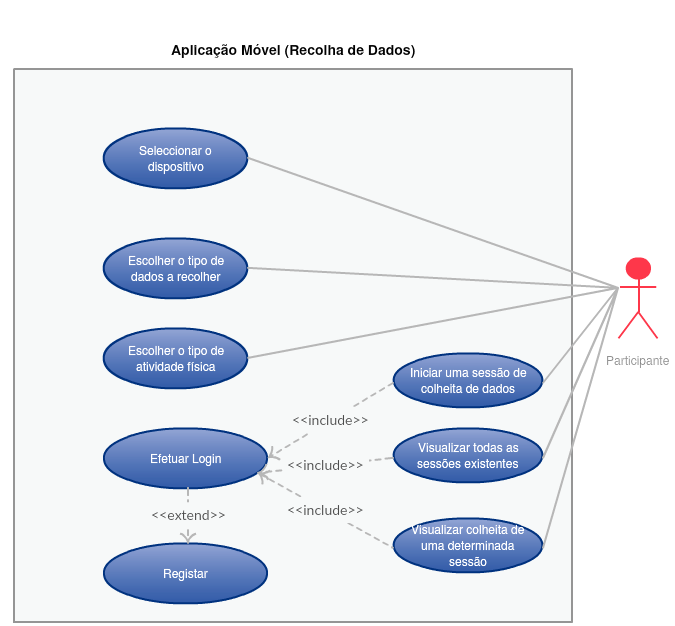
\includegraphics[width=0.9\textwidth]{imgs/app-and-usecase.png}
  \caption[Diagrama de casos de uso da aplicação móvel para recolha de dados]{Diagrama de casos de uso da aplicação móvel para recolha de dados}
  
  \label{f:usecaseandroidapp}
\end{figure}

\newpage


\begin{table}[H]
\centering

\begin{tabularx}{1\textwidth}{|p{4cm}|p{10.7cm}|}
\rowcolor[HTML]{FFCE93} \hline
\textbf{Caso de utilização} &  \textbf{Propósito do caso de utilização}  \\
\hline
Efetuar \textit{Login}  & O Participante deve conseguir entrar com a sua conta na aplicação móvel. \\ \hline

Registar & O Participante que vai participar no estudo pode criar uma nova  conta. \\ \hline

Escolher a relação temporal relativamente à atividade física & Consoante o tipo de atividade física que estiver a efetuar, o participante a sua relação temporal relativamente à atividade física. Tendo como exemplo a corrida, a relação temporal poderá ser entre as disponíveis: antes, depois, durante, em descanso\\ \hline

Escolher o tipo de dados a recolher & Tem que existir a possibilidade de filtrar o tipo de dados que são para ser recolhidos numa determinada colheita. Pode ocorrer a situação de recolher todos ao mesmo tempo. \\ \hline

Selecionar o dispositivo  & Para se conseguir efetuar a colheita dos dados um dispositivo válido tem que ser selecionado. \\ \hline

Iniciar uma sessão de colheita de dados & Pode iniciar uma nova colheita de dados. Esta nova colheita pode ser durante vários segundos, minutos e até horas. Apenas os dados escolhidos poderão ser guardados para posterior consulta. A colheita pode ser interrompida quando o participante quiser. \\ \hline

Visualizar todas as sessões existentes & O Participante pode visualizar todas as sessões de recolha dados. \\ \hline

Visualizar colheita de uma determinada sessão & O Participante ao escolher uma colheita das várias apresentadas e pode visualizar ao detalhe todos os dados recolhidos numa determinada sessão. \\ \hline    

\end{tabularx}

\caption{Breve descrição dos casos de utilização da aplicação de colheita de dados}
\label{t:android-usecase}
\end{table}

\section{Casos de Utilização na Revisão de Dados}

Na figura \ref{f:usecasewebapp} podemos visualizar todos os casos de uso (cenários-objetivo) da aplicação \textit{web}. O principal ator desta aplicação é o revisor/investigador que pode fazer uma revisão das várias sessões de recolha efetuadas pelos participantes. Uma breve descrição de cada caso de utilização é apresentada na tabela \ref{t:web-usecase}
\newpage
\begin{figure}[H]
  \centering
  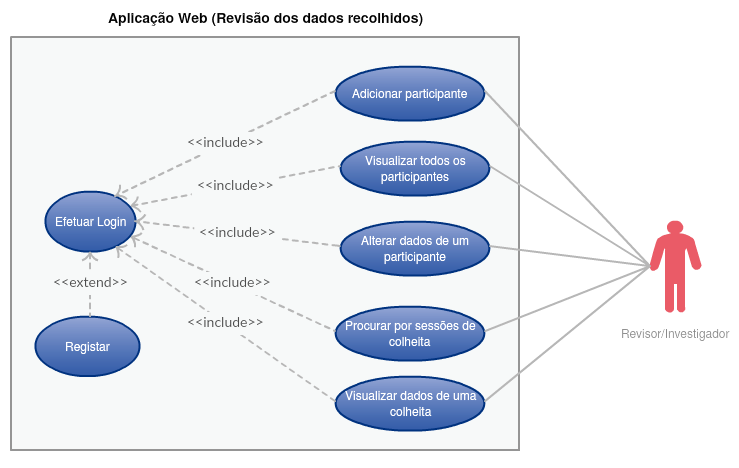
\includegraphics[width=0.9\textwidth]{imgs/app-web-usecase.png}
  \caption[Diagrama de casos de uso da aplicação \textit{web}]{Diagrama de casos de uso da aplicação \textit{web}}
  
  \label{f:usecasewebapp}
\end{figure}



\begin{table}[H]
\centering

\begin{tabularx}{1\textwidth}{|p{4cm}|p{10.7cm}|}
\rowcolor[HTML]{FFCE93} \hline
{\color[HTML]{000000} \textbf{Caso de utilização}} & {\color[HTML]{000000} \textbf{Propósito do caso de utilização}}  \\
\hline
Efetuar \textit{Login} & O Revisor deve conseguir entrar com a sua conta na aplicação \textit{web}. \\ \hline

Registar & O Revisor pode criar uma nova  conta. \\ \hline

Adicionar participante & O Revisor deve poder adicionar um novo participante como seu alvo de estudo.\\ \hline

Visualizar todos os participantes & O Revisor deve conseguir visualizar todos os participantes do seu alvo de estudo. \\ \hline

Alterar dados de um participante & A edição dos dados demográficos do participante deve ser possível. \\ \hline

Iniciar uma sessão de colheita de dados  & Pode iniciar uma nova colheita de dados. \\ \hline

Procurar por sessões de colheita & Relativamente a um participante deve ser possível  pesquisar colheitas efetuadas num determinado intervalo de tempo. \\ \hline

Visualizar dados de uma determinada sessão de colheita & O Revisor depois de pesquisar as sessões para um determinado intervalo, deve poder ver os dados recolhidos para cada uma das sessões. \\ \hline                        
\end{tabularx}

\caption{Breve descrição dos casos de utilização da aplicação de Revisão}
\label{t:web-usecase}
\end{table}

\cleardoublepage